%\documentclass[letterpaper, twocolumn]{article}
\documentclass[letterpaper]{article}

% Change the margins to 1 inch all around.
\usepackage[margin=1in]{geometry}

% font handling
%\usepackage{fontspec}

% for setting the linespace (\setstretch)
\usepackage{setspace}

% distance between the columns
\setlength{\columnsep}{1cm}

% for compactitem
\usepackage{paralist}

% for comments
\usepackage{verbatim}

\usepackage{booktabs}
\usepackage{longtable}
\usepackage{float}
\usepackage{graphicx}
\usepackage{hyperref}
\usepackage{listings}
\usepackage{amsmath}
\usepackage{tcolorbox}
\usepackage{amssymb}
\usepackage{parskip}


\usepackage[
	sorting=none,
	minbibnames=8,
	maxbibnames=9,
	block=space,
	backend=biber
]{biblatex}
\bibliography{bibliography}

\usepackage{lipsum}

\begin{document}

% Blue text box for answers.
\newtcolorbox{myanswerbox}[1][]{
  colback=blue!5!white, % Background color
  colframe=blue!75!black, % Bourder color
  fonttitle=\bfseries, %  Font style of the title
  title=#1, %  Title
  arc=0mm, %  Rounded corners
  #1
}

\lstset{
    language=Python,
    basicstyle=\ttfamily\small,
    keywordstyle=\color{blue},
    backgroundcolor=\color{lightgray}
}

%=============================
{
	\parindent0pt
	\setstretch{1.4}
	\ \\ \ \\ \ \\

	\hrulefill
	\vspace{0.0cm}
	\begin{spacing}{2.1}
	{	
		\flushleft
		\fontsize{22pt}{44pt}\selectfont 
		Homework 4: Games Theory
	}\\
	\textsc{Microeconomics - ECON 401A}
	\end{spacing}

	\ \\ \ \\
	{
		\setstretch{1.2}
		\textbf{Mauricio Vargas-Estrada}\\
		\textbf{Santiago Naranjo Manosalva}\\
		Master in Quantitative Economics\\
		University of California - Los Angeles\par
	}
	\ \\

	\hrulefill

}

%\newpage

%=============================
\section{Differentiated Bertrand}

Two firms $i \in \{1, 2\}$ sell imperfectly substitutable goods. They compete in Bertrand fashion by posting prices $p_i \in [0, 1]$. When they set prices $(p_1, p_2)$ the demand for firm 1’s good is $q_1(p_1, p_2) = 1 - p_1 + p_2$ and the demand for firm 2’s good is $q_2(p_2, p_1) = 1 - p_2 + p_1$. There are no costs of production, so the profit functions of the firms are
    
\[
\pi_1(p_1, p_2) = p_1(1 - p_1 + p_2)
\]
\[
\pi_2(p_2, p_1) = p_2(1 - p_2 + p_1)
\]

\begin{tcolorbox}
(a) Calculate the best-response functions $BR_1(p_2)$ and $BR_2(p_1)$ and draw them in $(p_1, p_2)$-space.
\end{tcolorbox}

For $BR_1(p_2)$:

\begin{eqnarray*}
\pi_1(p_1, p_2) &=& p_1(1 - p_1 + p_2)\\
\frac{d\pi_1}{dp_1} &=& 1 - 2p_1 + p_2 = 0
\end{eqnarray*}

From the F.O.C. we get:

\begin{eqnarray*}
p_2^* &=& 2p_1 - 1\\
p_1^* &=& \frac{1 + p_2}{2}
\end{eqnarray*}

In the same way, for $BR_2(p_1)$:

\begin{eqnarray*}
\pi_2(p_2, p_1) &=& p_2(1 - p_2 + p_1)\\
\frac{d\pi_2}{dp_2} &=& 1 - 2p_2 + p_1 = 0
\end{eqnarray*}

Therefore, from the F.O.C.:

\begin{eqnarray*}
p_1^* &=& 2p_2 - 1\\
p_2^* &=& \frac{1 + p_1}{2}
\end{eqnarray*}

\begin{myanswerbox}
    So the best response functions are:
    \begin{eqnarray*}
        p_1^* &=& \frac{1 + p_2}{2}\\
        p_2^* &=& \frac{1 + p_1}{2}
    \end{eqnarray*}
\end{myanswerbox}

\begin{figure}[htpb]
    \centering
    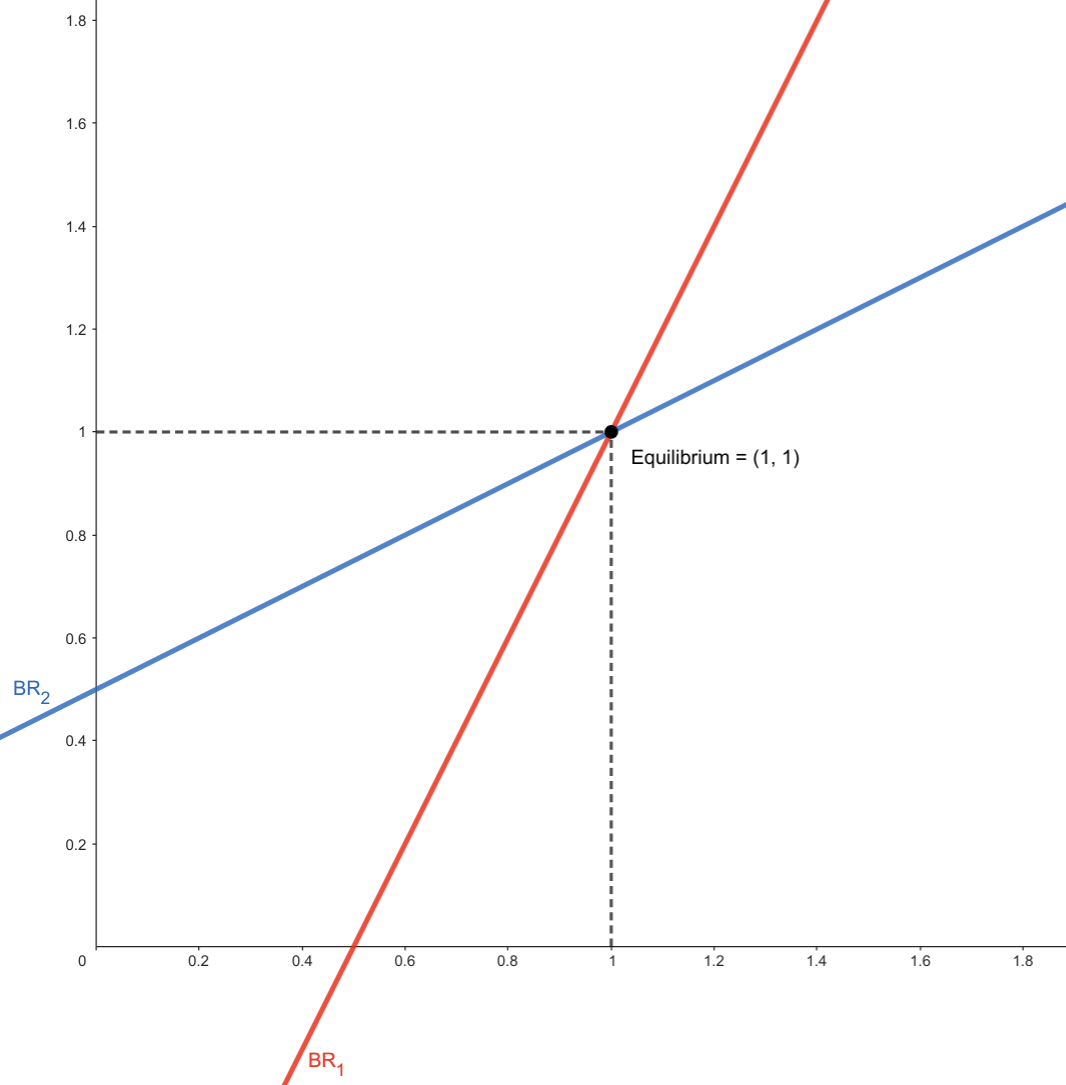
\includegraphics[scale=0.4]{plots/plot1.png}
    \caption{Best response functions}
    \label{fig:my_label}
\end{figure}

\begin{tcolorbox}
    (b) Calculate the Nash equilibrium prices $(p_1^*, p_2^*)$.
\end{tcolorbox}
    
The Nash equilibrium is the intersection of the best response functions, so:
    
\begin{eqnarray*}
p_1^* &=& \frac{1 + p_2}{2}\\
p_2^* &=& \frac{1 + p_1}{2}
\end{eqnarray*}
    
Substituting $p_1^*$ into $p_2^*$:
    
\begin{eqnarray*}
p_2^* &=& 2(2p_2 - 1) - 1\\
p_2^* &=& 4p_2 - 3\\
p_2^* &=& \frac{3}{3} = 1
\end{eqnarray*}
    
and substituting $p_2^*$ into $p_1^*$:
    
\begin{eqnarray*}
p_1^* &=& 2(1) - 1\\
p_1^* &=& 1
\end{eqnarray*}
    
\begin{myanswerbox}
    So the Nash equilibrium is $p_1^* = 1$ and $p_2^* = 1$.
\end{myanswerbox}
\section{Sales}

There are two firms $i \in \{1,2\}$ and three customers $\{A, B, C\}$. The firms choose prices $\{p_1,p_2\}$ simultaneously. Customer A only wants to buy from firm 1 and has a value of $v$. Customer B only wants to buy from firm 2 and has a value of $v$. Customer C values both products at $v$ and buys from the cheapest firm (and flips a coin if the prices are the same). There are no costs so, assuming $p_i \leq v$, firm $i$'s profits are

\[
\pi_i = 
\begin{cases} 
p_i & \text{if } p_i > p_j \\
\frac{3}{2}p_i & \text{if } p_i = p_j \\
2p_i & \text{if } p_i < p_j 
\end{cases}
\]

%%%%%%%%%%%%%%%%%%%%%%%%%%%%%%%%%%%%%%%%%%%%%%%%%%%%%%%%%%%%%%%%%

\begin{tcolorbox}
    \begin{enumerate}
        \item[(a)] Argue there is no pure strategy Nash equilibrium.
    \end{enumerate}
\end{tcolorbox}

Let's assume that there exists a Nash equilibrium in pure strategies. In this case, the problem for each firm is to maximize its profit given the optimal strategy of the opposing firm:

\begin{equation*}
    \max_{p_i} \pi_i(p_i, p_j^*)
\end{equation*}

Where $p_j^*$ is the optimal strategy of the opposing firm. In the case of firm 1, it maximizes its profit when:

\begin{equation*}
    p_1^* = p_2^* - \epsilon_1, \quad \epsilon_1 > 0
\end{equation*}

We need to add the $\epsilon_1$ term to ensure that $p_1^* < p_2^*$, since otherwise the profit of firm 1 would be $3/2 p_1^*$, and, therefore, firm 1 wouldn't be maximizing its profit.

Similarly, firm 2 maximizes its profit when:

\begin{equation*}
    p_2^* = p_1^* - \epsilon_2, \quad \epsilon_2 > 0
\end{equation*}

Substituting $p_2^*$ into the equation for $p_1^*$ and vice versa, it is obtained that:

\begin{equation*}
    p_1^* = p_1^* - \epsilon_2 - \epsilon_1 \implies \epsilon_1 + \epsilon_2 = 0
\end{equation*}

\begin{myanswerbox}
    Which is a contradiction, since $\epsilon_1, \epsilon_2 > 0$ in order to maximize their profits. Therefore, there does not exist a Nash equilibrium in pure strategies.
\end{myanswerbox}

%%%%%%%%%%%%%%%%%%%%%%%%%%%%%%%%%%%%%%%%%%%%%%%%%%%%%%%%%%%%%%%%%

\begin{tcolorbox}
    \begin{enumerate}
        \item[(b)] We now derive the symmetric mixed strategy equilibrium. Suppose both firms choose random price with cdf $F(p)$ and support $[p,\bar{p}]$. Argue that $\bar{p} \leq v$. Write down firm 1's profit from price $p \in [p,\bar{p}]$.
    \end{enumerate}
\end{tcolorbox}

The profit function for firm 1, given the optimal strategy of firm 2, is:

\begin{equation*}
    \pi(p) = p (1 - F(p)) + p F(p)
\end{equation*}

Because $F(p)$ represents the probability to choose a price lower that $p$, and $1 - F(p)$ the probability to choose a price higher than $p$.

\begin{eqnarray*}
    \pi(p) &=& p (1 - F(p)) + 2pF(p)\\
    \pi(p) &=& p - pF(p) + 2pF(p)\\
    \pi(p) &=& p (1 + F(p))
\end{eqnarray*}

\begin{myanswerbox}
    So the profit function for firm 1 (and 2) in terms of the cdf $F(p)$ is:

    \begin{equation*}
        \pi(p) = p \left(1 +  F(p) \right)
    \end{equation*}

    Consumers only buy if the price is lower than their valuation, so the maximum price a company can charge is \( v \). If it charged more, consumers would not buy and the company would not make any profit. Therefore, \( \bar{p} \leq v \).
\end{myanswerbox}

%%%%%%%%%%%%%%%%%%%%%%%%%%%%%%%%%%%%%%%%%%%%%%%%%%%%%%%%%%%%%%%%%

\begin{tcolorbox}
    \begin{enumerate}
        \item[(c)] Argue that $\bar{p} = v$ in equilibrium.
        \item[(d)] Derive the distribution of prices $F(p)$ in equilibrium. What is the support of prices $[p, \bar{p}]$?
    \end{enumerate}
\end{tcolorbox}

Because the purpose of the firms is to make profits, the lower bound of the support of prices is $p = 0$, so in that case the profit of firm 1 is:

\begin{equation*}
    \pi(0) = 0 \left(1 +  F(0) \right) = 0
\end{equation*}

In the case of the upper bound, the profit of firm 1 is:

\begin{equation*}
    \pi(\bar{p}) = \bar{p} \left(1 +  F(\bar{p}) \right)
\end{equation*}

If this is an equilibrium, then both firms should be indifferent between choosing this price and any other price in the support, including the case where both firms choose the same price. When both firms choose the same price, the profit of firm 1 is:

\begin{eqnarray*}
    \pi(\bar{p}) = \bar{p} \left(1 +  F(\bar{p}) \right) &=& \frac{3}{2} \bar{p}\\
    1 +  F(\bar{p}) &=& \frac{3}{2}\\
    F(\bar{p}) &=& \frac{1}{2}\\
\end{eqnarray*}

\begin{myanswerbox}[Answer to (d)]
    To allow this possibility, the cdf $F(p)$ should be from a discrete distribution with a mass of $1/2$ at $\bar{p}$, and a mass of $1/2$ at $p = 0$, so the support of prices is $[0, \bar{p}]$ distributed according to a Bernoulli with parameter $1/2$.
\end{myanswerbox}

\begin{myanswerbox}[Answer to (c)]
    In question (b) we argued that \( \bar{p} \leq v \) to ensure consumers buy the products, but because the distribution of prices follows a Bernoulli with parameter \( 1/2 \), the only possible way to cover the entire support range is when \( \bar{p} \) is \( v \).
\end{myanswerbox}

\section{Double Marginalization}

A manufacturer M sells his product to consumers through a retailer R. First, the manufacturer sets a wholesale price $w \geq 0$. The retailer sees this and chooses the final price p $\geq$ w. The demand function is $Q(p) = 1 - p$. For simplicity, assume the manufacturer and retailer have zero cost. The profit functions are thus given by $\pi M = w(1 - p)$ for the manufacturer and $\pi R = (p - w)(1 - p)$ for the retailer.

\begin{tcolorbox}
    (a) Given w what is the optimal price p of the retailer?
\end{tcolorbox}

\begin{eqnarray*}
\pi_R &=& (p - w)(1 - p)\\
\pi_R &=& p-p^2-w+wp\\
\frac{d\pi_R}{dp} &=& 1-2p+w = 0\\
\frac{1+w}{2} &=& p\\
\end{eqnarray*}

\begin{myanswerbox}
    The optimal price of the retailer is $\frac{1+w}{2}$.
\end{myanswerbox}

\begin{tcolorbox}
    (b) Using backwards induction, what is the optimal wholesale price w of the manufacturer?
\end{tcolorbox}

\begin{eqnarray*}
\pi_M &=& w(1 - p)\\
\frac{1+w}{2} &=& p\\
\pi_M &=& w(1 - \frac{1+w}{2})\\
\pi_M &=& (w - \frac{w+w^2}{2})\\
\pi_M &=& w - \frac{w}{2}-\frac{w^2}{2}\\
\frac{d\pi_M}{dw} &=&  1 - \frac{1}{2}-\frac{2w}{2}=0\\
w&=&\frac{1}{2}=0.5\\
p&=&0.75
\end{eqnarray*}

\begin{myanswerbox}
    The optimal wholesale price of the manufacturer is 0.75.
\end{myanswerbox}

\begin{tcolorbox}
    (c) What are the firms' profits in equilibrium?
\end{tcolorbox}

\begin{eqnarray*}
\pi_R &=& (p - w)(1 - p)\\
\pi_R &=& (0.75 - 0.5)(1 - 0.75)\\
\pi_R &=& (0.25)(0.25)\\
\pi_R &=& 0.0625\\
\\
\pi_M &=& w(1 - p)\\
\pi_M &=& 0.5(1 - 0.75)\\
\pi_M &=& 0.5(0.25)\\
\pi_M &=& 0.125
\end{eqnarray*}

\begin{myanswerbox}
    The firms' profits in equilibrium are $\pi_R = 0.0625$ and $\pi_M = 0.125$.
\end{myanswerbox}

\begin{tcolorbox}
    (d) Now assume that manufacturer and retailer integrate vertically and charge a price p to maximize joint profits $\pi(p) = p(1 - p)$. What is the optimal price p?
\end{tcolorbox}

\begin{eqnarray*}
\pi(p) &=& p(1 - p)\\
\pi(p) &=& p - p^2\\
\frac{d\pi(p)}{dp} &=& 1 - 2p=0\\
p &=& \frac{1}{2}\\
\pi(p) &=& 0.25\\
\end{eqnarray*}

\begin{myanswerbox}
    The optimal price is 0.5 and the joint profit is 0.25.
\end{myanswerbox}

\begin{tcolorbox}
    (e) How do industry profits in the vertically integrated firm compare to the equilibrium in (c)? Explain the difference.
\end{tcolorbox}

\begin{eqnarray*}
\pi_R + \pi_M= 0.0625 + 0.125= 0.1875\\
\pi(p) = 0.25\\
\end{eqnarray*}

\begin{myanswerbox}
    The increase in total profit due to vertical integration (from  0.1875 to 0.25) exemplify the economic theory that suggests vertical integration can yield advantages by mitigating the inefficiencies linked to double marginalization, thereby improving the integrated entity's profitability.
\end{myanswerbox}
\section{Tax Competition}

\begin{tcolorbox}
    Each US state independently chooses its own taxes, seeking to attract firms and workers from other states. For example, Kansas famously slashed its income tax rates in 2012; the Governor claimed this would "bring businesses from across the nation to the Midwest" and that he would "keep pruning state government any place that we can" in order to balance the budget. Is such tax competition good for the US population as a whole (in the same way competition across firms is good for welfare) or do states impose negative externalities on one another?

\end{tcolorbox}

Tax competition allows state governments to compete by offering incentives to investors or controlling internal markets. Certain businesses and individuals would face obstacles as a result of this competition, but others would be encouraged to enter the market. These kinds of regulations allow governments to control their own markets to suit their own requirements.

The following is a comparison of the advantages and disadvantages of tax competition and its possible effects for the US population:

Advantages:

\begin{itemize}
\item As a result of the tax structures offered, consumers will have the freedom to choose between various states, thus increasing their utilities according to their initial preferences.
\item The effectiveness and innovation of policies aimed at increasing incentives for investment in different nations would be increased by establishing a competitive market.
\item States would have to maintain high fiscal discipline, evident in the management of finances before society, due to concern about losing business.
\end{itemize}

Disadvantages:

\begin{itemize}
\item The uneven distribution of resources and wealth among the states as a result of each state's failure to provide investors with the same incentives.
\item States will likely keep competing with one another to provide bigger incentives, which can result in lower taxes and less money for public services.Reduced financing for basic public services may have long-term consequences for growth, impacting infrastructure, health, safety, and education standards, as well as perhaps driving migration to other states.
\end{itemize}

In conclusion, permitting tax rivalry across states may spur innovation and growth, but such competition needs to be carefully managed to prevent unfavorable effects. It is imperative that policymakers compete to satisfy and safeguard the interests and well-being of societies while also being cognizant of the demands of individual states.
\section{Ransoms}

\lipsum[10]

\end{document}
